\chapter{Formal languages}
\section{Overview}
A formal language is an abstract language that, unlike concrete languages, often does not focus on communication but on mathematical use. A formal language consists of a certain set of symbol strings (generally strings) that can be assembled from a set of characters or symbols. Formal languages are used in linguistics, logic and theoretical computer science.

Formal languages are suitable for the (mathematically) precise description of the handling of character strings. For example, data formats or entire programming languages can be specified. Together with a formal semantics, the defined character strings have a meaning. With a programming language, a programming instruction (as part of the formal language) can be assigned a unique machine behaviour (as part of the semantics).

Based on formal languages, however, it is also possible to define logic calculi with which one can draw mathematical conclusions. In conjunction with formally defined programming languages, calculi can help to check programs for their correctness.

All major information here are from the book \cite{rechenberg_compiler-generator_1988} written by Rechenberg Peter and Mössenböck Hanspeter. This book describes in detail how a compiler works, especially with the usage of formal grammars and syntax analysis 
\section{Alphabets and Strings}
\subsection{Alphabet}
An alphabet (sometimes called a Vocabulary) is a non-empty and finite set of elements. Alphabets are often denoted by upper-case letters $A$ or $V$ and sometimes as upper-case Greek letters like $\Sigma$. Examples of common alphabets are e.g. the machine text alphabet ASCII or the binary bit $0$ or $1$.
\subsection{String}
A string (or word) is a finite sequence of elements, called symbols or letters selected from a particular finite set which is the alphabet.
The length of a string $\omega$ is denoted as $|\omega|$ which gives the number of symbols in the string. The empty string is a special word which has no symbols and is denoted by $\varepsilon$ or $\lambda$. This means a string $\omega$ is called an empty string if $|\omega|=0$.
\subsection{Concatenation}
The basic operation of strings is concatenation, i.e., writing strings as a junction. Let $\omega_1$ and $\omega_2$ be two strings. Then the concatenation of $\omega_1$ and $\omega_2$ makes a new string $\alpha$ containing all the symbols of $\omega_1$ in order followed by all symbols of $\omega_2$ in order. This is usually written as $\alpha=\omega_1\omega_2$.
Concatenations in the alphabet $\{x, y, z\}$ can be:
\begin{align*}
\omega_1&=xxzyyx	& \omega_2&=zxxz	& \omega_1\omega_2&=xxzyyxzxxz\\
\omega_1&=xxzyyx	& \omega_2&=\varepsilon	& \omega_1\omega_2&=xxzyyx\\
\omega_1&=\varepsilon	& \omega_2&=zxxz	& \omega_1\omega_2&=zxxz
\end{align*}

The concatenation on an alphabet has two important properties:

\begin{itemize}
	\item Assiciativity: $\omega_1(\omega_2\omega_3)=(\omega_1\omega_2)\omega_3$
	\item An identity element $\varepsilon$: i., e., $\omega\varepsilon = \varepsilon\omega = \omega$
\end{itemize}

In some cases string notation can be simplified by the following rules: 

$a^n$ \qquad For strings containing $n$ same symbols, e.g., $a^3=aaa$

$\varepsilon$\qquad\quad The empty string containing null symbols

$a^+$ \qquad For strings with set of $(a^n:n\geq1)$, e.g., $a^+=\{a, aa, aaa, aaaa, \ldots\}$

$a^*$ \qquad For strings with set of $(a^n:n\geq0)$, e.g., $a^*=\{\varepsilon, a, aa, aaa, aaaa, \ldots\}$
 
\section{Production Rules and Grammars}
\subsection{Kleene Star}
The Kleene star set $\Sigma^*$ of an alphabet $\Sigma$ is a language that contains all the words of the alphabet. It can be defined by means of structural induction. 
Firstly, in the beginning of the induction the empty word $\varepsilon$ is defined. Then in the induction step it is defined that each string is being one element in the Kleene star set.
To define the sets $\Sigma_i$ recursively, we use the following components:
\begin{itemize}
\item \textbf{Basis Clause: }$\Sigma_0 = \{\varepsilon\}$ 
\item \textbf{Inductive Clause: }$\Sigma_{i+1} = \{\omega v \mid \omega\in\Sigma_{i-1}\wedge v\in\Sigma\}$
\end{itemize}
The Kleene star is defined then by $\Sigma^* = \bigcup\limits_{i\in\mathbb{N_0}} \Sigma_{i}$
In other words, the Kleene Star of an alphabet is the set of all strings that can be built out of an alphabet.

The Kleene star set $L^*$ of a language $L$ is the union of all its potential languages (repeated concatenation of languages):
$$L^* = \bigcup\limits_{i\in\mathbb{N_0}} \L^{i}$$
Where $L^0 = \{\varepsilon\}$ and $\L^{n+1} = L^nL$. 

\subsection{Production Rule}
A grammar rule has the form:
$$X \rightarrow \alpha \qquad \quad \textrm{With} \quad X \in V \quad \textrm{and} \quad \alpha \in V^*$$
It is read ``$X$ is defined as $\alpha$'' or ``$X$ can be replaced by $\alpha$'' and means that in a string containing $X$, $X$ can be replaced by $\alpha$. Several rules with the same left side such as:

$X \rightarrow \alpha_1$

$X \rightarrow \alpha_2$

$X \rightarrow \alpha_3$

are usually grouped together by separating the alternatives with the character ``$\mid$'':
$$X \rightarrow \alpha_1 \mid \alpha_2 \mid \alpha_3$$
All symbols appearing on the left side of a production rule or generally a grammar are non-terminals $V_N$ and all others are terminal symbols $V_T$. The rules describe substitutions of non-terminal symbols by strings. In the formal language theory these substitutions are called production rules. A grammar is defined by production rules that indicate which symbols can replace which other symbols. These rules can be used to generate strings or parse them.

Parsing is the process of recognizing an utterance (a string in natural languages) by breaking it up into a series of symbols and analysing them with the grammar of the language. Most languages have structured the meanings of their utterances according to their syntax.

To create a string in the language, we start with a string that consists only of a start symbol. This start symbol $S$ appears on at least one left side of the production rules. All symbols on the left and right sides are the Vocabulary.
From the starting symbol $S$, each symbol will be replaced repeatedly by strings, according to the rules of the grammar, until a string is created which contains only terminal symbols.

\subsection{Definition of a Grammar}
A grammar $G(S)$ is a finite, non-empty set of production rules. The rules describe how to build strings from the alphabet of the language that are valid according to the syntax of the language. A grammar does not describe the meaning of the strings or what can be done with them in any context, just their form.

\subsection{Syntax of formal grammars}
A formal grammar is represented by the 4-tuple $G=(N,\Sigma,P,S)$ wherein:
\begin{itemize}
\item $N$: a finite set of non-terminal symbols that is separated from the $G$ formed strings.
\item $\Sigma$: a subset of $V$, also called alphabet whose elements are called terminal symbols 
\item $P$: a finite set of production rules where each rule has the form: $(\Sigma \cup N)^{*}N(\Sigma \cup N)^{*}\rightarrow (\Sigma \cup N)^{*}$
\item $S \in N$: the start symbol
\end{itemize}
The set $N = V \setminus T$ is the set of non-terminal symbols (also called meta-symbols), in particular the start symbol belongs to it. The word on the left side of the rule pairs may not consist exclusively of terminal characters, which can also be expressed by a concatenation: $(V^* \setminus T^*) = V^*NV^*$.

\subsection{Terminal and Non-Terminal Symbols}
The grammatical structure of a statement, a program or generally of a string is a tree, the so-called syntax tree. There are two types of symbols:
\begin{itemize}
\item \textbf{Terminal symbols: }these are the symbols of the sentence itself, i.e. the symbols that can not be further decomposed. In other words they are the ``leaves'' of the tree and are donated with lower-case letter. 
\item \textbf{Non-Terminal symbols: }these are all other symbols with upper-case letters.
\end{itemize}
With $V=V_N \cup V_T$ we denote the union of the alphabets of terminal and non-terminal symbols.
Each tree contains an excellent non-terminal symbol, the start symbol or the root from which the whole tree originates. The allowed structures of syntax trees and thus sentences of a formal language are described by ``grammars''.

\subsection{Derivation}
Let a string $\alpha$ generating directly a string $\beta$, written $\alpha \Rightarrow \beta$. Given a formal grammar $G$ with a rule $A \rightarrow \varphi$. If there are the strings $\omega_1$ and $\omega_2$ with the definition $\alpha = \omega_1A\omega_2$, then we can obviously generate a new string $\beta = \omega_1\varphi\omega_2$.
 
A sequence of direct generations is described with the symbols $\Rightarrow^+$ and $\Rightarrow^*$. When a string $\alpha$ produces another string $\beta$ with the form $\alpha \Rightarrow^+ \beta$ then it is about a multiple string generation. A sequence of applications of the rules of a grammar that produces a finished string of terminals is mostly called as derivation. 
$$\alpha = \omega_0 \Rightarrow \omega_1 \Rightarrow \omega_2 \ldots \Rightarrow \omega_n = \beta \qquad \quad \textrm{with} \quad n \geq 1$$ 
In case, that $\alpha \Rightarrow^+ \beta$ or $\alpha = \beta$ we write $\alpha \Rightarrow^* \beta$. This means $\alpha$ generates or is equal to $\beta$.

\subsection{Example}
Given the grammar $G = (\{S,A,B\},\{a,b,c\},P,S)$ with the non-terminal symbols $S,A,B,$ the terminal symbols $a,b,c$ and the production rule set $P$:

$S \rightarrow Ac$

$A \rightarrow aB \mid BBb$

$B \rightarrow b \mid ab$

Now the following types of strings can be generated by derivation:

\begin{tabular}{llll}
$S \Rightarrow Ac$ & $\Rightarrow aBc$ & $\Rightarrow abc$ & \\
 & & $\Rightarrow aabc$ & \\
 & $\Rightarrow BBbc$ & $\Rightarrow bBbc$ & $\Rightarrow bbbc$ \\
 & & & $\Rightarrow babbc$ \\
 & & $\Rightarrow abBbc$ & $\Rightarrow abbbc$ \\
 & & & $\Rightarrow ababbc$ \\
\end{tabular}

Therefore it is $L(G) = \{``abc", ``aabc", ``bbbc", ``babbc", ``abbbc", ``ababbc"\}$

If $G(S)$ is a formal grammar with a start symbol $S$ then the set $$L(G(S)) = \{\alpha : S \Rightarrow^* \alpha \wedge \alpha \in V^{*}_{T}\}$$
is called the language of $G(S)$.

\section{Languages}
Formally, a language $L$ is defined as a set of strings over some finite alphabet. Specific examples of languages are finite languages with a finite number of words.

For languages we use the usual set-theoretic notations like:
\begin{itemize}
\item $\subseteq$ (inclusion), 
\item $\supseteq$ (proper inclusion), 
\item $\cup$ (union), 
\item $\cap$ (intersection), 
\end{itemize}
A formal language $L$ over an alphabet $\Sigma$ is an arbitrary set of words about $\Sigma$, i.e., $L \subseteq \Sigma^*$.

If a string $\omega$ belongs to a language $L$ it is denoted by $\omega \in L$, as usual. There are also ``negated'' relations such as $\not\subseteq$, $\not\subset$ and $\not\in$.

Examples of languages:
\begin{itemize}
\item Above the letter A-Z including umlauts and punctuation marks. The set of all
grammatically correct German sentences
\item The grammar G(Java) defining the programming language Java. L(G(Java)) is then the set of all syntactically correct Java
programs
\item Above the ASCII character set. The set of all C programs
\end{itemize}

\section{Syntax Notations}
Syntax notations are compact formal meta-languages for representing context-free grammars. This includes the syntax of common higher-level programming languages. It is also used for the notation of instruction sets and communication protocols.

There are essentially three methods for the syntax description and they will be explained in the following sections. They describe the syntax as a grammar in the form of so-called syntax rules. They form a well-understood formal system and find their justification in the theory of formal languages.

\subsection{Classical}
In computer science different spellings are used for grammar rules. Nevertheless, the previously used syntax has the following identifiers:
\begin{itemize}
\item Terminals in lower-case letters
\item Non-terminals in upper-case letters
\item Separator: $\rightarrow$ 
\item Alternatives: $|$
\end{itemize}
The language of propositional logic is defined with the classical notation system of formal languages as follows.

\begin{tabular}{lll}
$F$ & $\rightarrow$ & $I |\neg F |(F \wedge F) |(F \vee F)$\\
$I$ & $\rightarrow$ & $a | b | c$ \\
\end{tabular}
\subsection{EBNF}
The extended Backus-Naur form meta-syntax notations is a very commonly used form for defining grammars that is equivalent to the syntax diagrams and substitution rules. It is very similar to the previously used spelling in the productions, but has the advantage that it is easier machine-readable.
The EBNF has the following rules:
\begin{itemize}
\item Terminals under double quotes
\item Non-terminals in meaningful words written in camel case
\item Separator: $=$ 
\item Alternatives: $|$
\item Each rule ends with a period 
\item Options: $[A]$ means $A$ or empty $\epsilon$
\item Repetition: $\{A\}$ means $\epsilon$ or $A$ or $AA$ or $AAA$ \ldots
\item Brackets for grouping
\end{itemize}
As an example we can take a look at the EBNF syntax of the expressions in the programming language Modula 2 from \cite{rechenberg_compiler-generator_1988}.

\begin{tabular}{lll}
$expression$ & $=$ & $ [``+" |``-"] term \{(``+" |``-") term\}$\\
$term$ & $=$ & $factor \{(``*" |``/") factor\}$ \\
$factor$ & $=$ & $c |v |``(`` expression ")"$ \\
\end{tabular}

\subsection{Syntax Diagrams}
A syntax diagram is used in theoretical computer science to graphically represent the syntax of a rule set. In particular, formal languages up to the class of context-free languages, and thus the syntax of programming languages due to the subset property, can be represented in a syntax diagram.

Each extended Backus-Naur form (EBNF) can be converted with the help of enclosed translation one on one in a syntax diagram.
Figure~\ref{fig:syntaxDiagram} shows how the previous EBNF example could look like after a success translation into a syntax diagram.

\begin{figure}[h] 
	\centering
	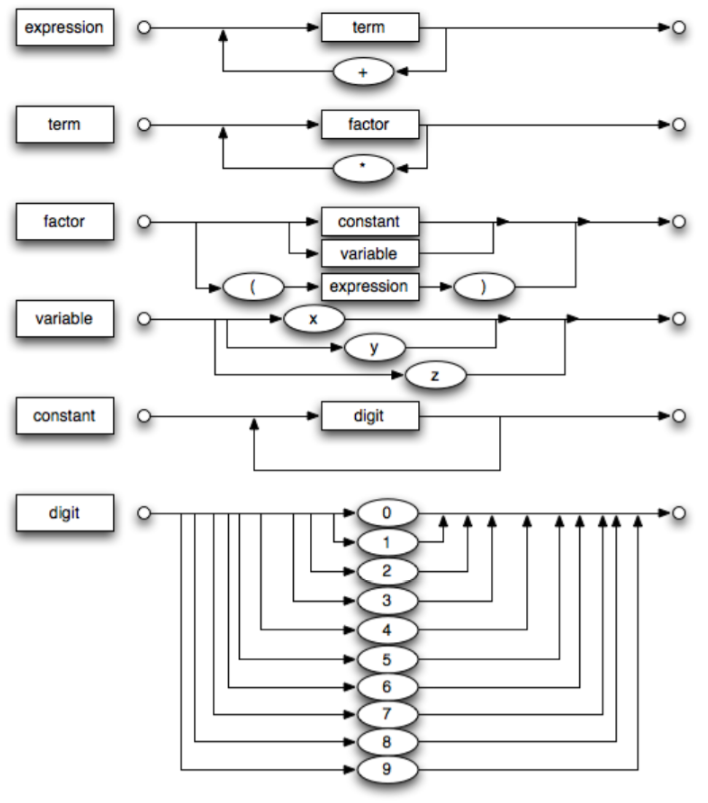
\includegraphics[scale=.68]{images/syntaxDiagram.png}
	\caption{Example of a syntax diagram}
	\label{fig:syntaxDiagram}
\end{figure}
